\section{Data integrity and evaluation}
\label{app:integrity}
\label{app:evaluation}
The study fits models on 112 people (692 motions, 1,645 windows) and evaluates them on 14 different development people (155 windows). Every edit, mirror, view, and corrupted observation inherits its source person's split. Known duplicate motion hashes cannot cross splits. Training excludes the 15$\dg$ edit and ViTPose inputs. Their evaluation still uses the same development people; no locked-person confirmation was completed.

\begin{figure}[h]\centering
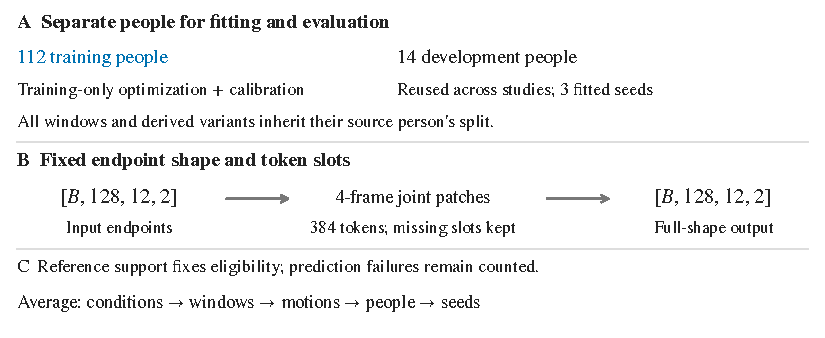
\includegraphics[width=\linewidth]{figures/protocol.pdf}
\caption{Data preparation and evaluation protocol. Source-person identity determines the split before variants are created. Four-frame patches regroup the fixed joint/time array without dropping missing slots. Fitting and loss calibration use training pairs; evaluation retains reference-eligible failures and averages repeated observations before people. The development cohort is reused across all stages.}
\label{fig:protocol}
\end{figure}

\paragraph{What stays fixed.} Preparation resamples motion to 25 Hz, selects nonoverlapping windows, and creates synthetic observations; it changes values and record counts. The model preserves the resulting $[B,128,12,2]$ coordinate layout, with confidence and availability $[B,128,12]$ and timestamps $[B,128]$. Each token packs four frames of one joint; decoding restores their original positions. Neither leg is separately time-warped or rescaled. Input naming swaps permute observations and their confidence/availability together while reference anatomy stays fixed.

\paragraph{What fitting can access.} Student inputs contain observed coordinates, native confidence, availability, and time. Projected references supply training targets and teacher inputs. Origin and isotropic scale use available, artificially unmasked observations only; references share that transform. Optimization and gradient calibration use training pairs. Data-integrity checks may read development references for consistency and identity, but these references do not enter fitting losses. Locked-confirmation participants are excluded from fitting. Unknown person aliases and overlap with pose estimators' training data remain possible.

\paragraph{What counts in evaluation.} Reference support is shared across variants of each source window. Angular scoring requires finite reference geometry, segments at least two pixels long, at least 16 frames, and 80\% coverage. Prediction failures remain eligible and receive the declared costs. Means average conditions within windows, windows within motions, motions within people, then seeds. Nonheld/held groups retain 2:1 response weighting and 4:1 endpoint weighting; extra renderings do not increase the participant count.

\paragraph{How uncertainty is calculated.} Core and feature-response comparisons use 2,000 paired bootstrap draws (RNG seed 731), independently resampling 14 people and three seeds. Repair first averages each person's differences over seeds, then uses $\bar d\pm t_{.975,13}s_d/\sqrt{14}$; its crossed bootstrap is a sensitivity check. This person-$t$ interval conditions on the fitted seeds. Neither procedure accounts for adaptive reuse of development results.

\clearpage
\section{Reproducible training specification}
\label{app:methods}
\label{app:optimization}
The full technical supplement retains loss reductions, masking rules, and optimizer equations. The specifications below identify the fitted procedures and the controls needed to interpret them. Recorded experimental configurations and training logs establish the completed settings.

\paragraph{Observations and geometry.} Walking candidates are screened from AMASS filenames and projected geometry, without clinical verification. Right-knee edits of 0, 5, 10, or 15 degrees are gated by an ankle-height proxy and taper at window boundaries. Editing precedes physical mirroring. Cameras, fitted across each window's original, edited, and mirrored motions, remain fixed; oblique and side views use 45 and 90 degrees. References are projected body-model joints, including image-hidden joints. Nominal 3D edit angles need not equal projected response changes.

\paragraph{Model and masking.} Five channels per frame (two coordinates, confidence, availability, time) give a 20-dimensional joint patch, mapped to width 96. The encoder has four layers and four heads; the predictor has two layers. Joint and time identifiers persist through masking. Graph--time masks hide connected joint regions and time intervals, using about half the available tokens while retaining context. Unavailable slots remain in the 384-token sequence. The readout uses LayerNorm, a $96\to96$ linear map, GELU, and a zero-initialized $96\to8$ map. It adds coordinate corrections where observed and predicts absolute coordinates where missing.

\paragraph{Losses and support.} Coordinate fitting averages squared normalized error over reference-valid coordinates, then endpoints equally. The base feature objective uses centered teacher--student cross-entropy (temperatures 0.06/0.1) plus $0.05L_{\rm VICReg}$; it follows the DINO mechanism rather than I-JEPA's regression. VICReg uses translated views with invariance/variance/covariance weights 25/25/1. Endpoint and delta auxiliaries (Equation~\ref{eq:feature}) average common queries within pairs, then pairs equally; all four reference frames must be valid in both patches. Shuffled-reference pretraining instead uses another window of the same person, preserving observation conditions and endpoint role.

The original readout minimizes $L_x+L_s+L_g$, low scalar uses $L_x+0.1L_s+L_g$, and dense uses $L_x+\lambda_dL_d+L_g$. Both angular terms use squared errors divided by $180^2$. Dense supervision averages the squared error between predicted and reference paired angle changes over common supported legs and timestamps. Geometry loss penalizes predicted segments shorter than two pixels on reference-defined support. Thus the original coordinate-to-change comparison adds two penalties together. Repair keeps geometry and coordinate terms fixed.

\paragraph{Updates and calibration.} Seeds are 17, 29, and 43. Pretraining and frozen readout fitting each use 2,000 updates; direct fitting uses 4,000 joint updates. Batch size is 16; draws sample person, motion, window, then pair uniformly at each level. AdamW uses peak rate $3\times10^{-4}$, 5\% warmup, cosine decay, weight decay 0.01, and gradient-norm clipping at one. Teacher momentum rises from 0.99 to 0.999; the center momentum is 0.9. Fresh readouts share initialization across arms (seed $+100003$). Equal update totals do not match encoder adaptation or supervised exposure.

On 32 training batches at seed-17 initialization, the shared feature coefficient $\lambda_J=0.0126468$ gives endpoint gradients 10\% of base RMS magnitude and delta 0.001303714\%, before clipping. The six new feature fits clip 11,999 of 12,000 updates. For each repair encoder/seed, 32 training batches instead calibrate $\lambda_d$ to low scalar's initial gradient magnitude. These records describe initialization and clipping; they do not establish later influence, convergence, or the cause of a ranking.

\clearpage
\section{Primary questions and supporting comparisons}
\label{app:inventory}
Each primary comparison estimates a paired difference in measurement error between two fitted procedures. Figure~\ref{fig:questions} summarizes the three declared primary contrasts. For each, gain is comparator error minus candidate error after the recorded averaging. A retrospective no-benefit null is $H_{0,j}:\mu_j\leq0$, against $\mu_j>0$. We retain two-sided 95\% intervals; this notation implies neither preregistration nor a new one-sided test.

\begin{figure}[h]\centering
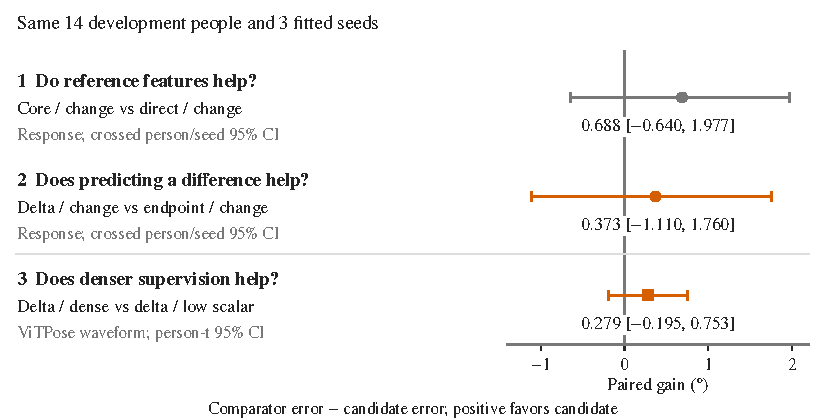
\includegraphics[width=\linewidth]{figures/study-questions.pdf}
\caption{Three sequential questions, with their recorded primary gains and 95\% intervals. The first two concern pooled response error and use crossed person/seed bootstraps. The third concerns ViTPose waveform error and uses a person-$t$ interval after seed averaging. Positive values favor the candidate. Different outcomes and inference procedures are separated; there is no pooled effect. Every interval spans zero, leaving each primary benefit unresolved. All comparisons reuse 14 development people and three fitted seeds.}
\label{fig:questions}
\end{figure}

\paragraph{Baselines establish the scale.} Zero response has pooled error 5.81$\dg$ and supplies no trajectory or anatomical assignment. Unchanged observations score 12.69$\dg$ response and 18.57$\dg$ waveform error; direct coordinate fitting improves these to 7.54$\dg$ and 12.07$\dg$. The initial primary instead compares core JEPA with direct fitting under the original change objective. Replacing its comparator with direct coordinate fitting would change the question.

\paragraph{Controls constrain the feature claim.} Figure~\ref{fig:restoration} retains all eight encoders/training procedures with both readout objectives, including initialized features, shuffled references, and coordinate pretraining. These controls ask whether useful information comes from fitting a readout, preserving correspondence, or reconstructing coordinates. They are diagnostic variants within one cohort. The complete means remain in the technical supplement; no configurations are averaged into a new method.

\paragraph{Follow-ups change the interpretation.} Under coordinate-only readouts, delta has higher response error than endpoint (10.94$\dg$ versus 10.23$\dg$), reversing their ordering under the original change objective. The interaction remains uncertain. Adding the original change package increases waveform means in all eight procedures, by 4.39--7.21$\dg$. On ViTPose, lowering delta's scalar weight improves waveform error by 3.70$\dg$ [2.58, 4.81]$\dg$; the smaller additional dense-supervision benefit is the third primary above. Reduced waveform error does not establish preserved response accuracy. These exploratory comparisons explain the next question without supplying independent confirmation.

\clearpage
\section{Diagnostics and reproducibility}
\label{app:strata}
\label{app:cost}
\label{app:failures}
\label{app:repair}
\label{app:reproduction}
\label{app:journey}
\paragraph{Observation conditions.} Main Table~\ref{tab:strata} shows every clear/occluded by nominal-edit group for the task baselines and the focal direct, endpoint, and delta procedures. Direct coordinate fitting beats zero response in both clear-image groups and neither occluded group; endpoint and delta with change readouts exceed zero in all four. The supplement retains all 16 variants in all four groups and all six visibility-by-estimator groups. The 5/10$\dg$ versus 15$\dg$ distinction describes nominal edits, not bins of true projected response. The available aggregate results omit the per-pair values required for that latter analysis.

\paragraph{Failure costs and denominators.} For $\theta\in[0,180]\dg$, excursion lies in $[0,180]\dg$, signed asymmetry in $[-180,180]\dg$, and paired response in $[-360,360]\dg$. The maximum discrepancy between valid responses is therefore 720$\dg$, the original failure cost. Waveform failures cost 180$\dg$. Equation~\ref{eq:cost} keeps failed cases in the population. If $U$ is the unconditional successful-error contribution and $f$ the weighted failure fraction, $U/(1-f)$ is a conditional error; adding it to failure cost would mix denominators.

Figure~\ref{fig:reliability} retains every examined cost (0, 180, 360, 720$\dg$). The endpoint-minus-delta gain ranges from 0.10$\dg$ to 0.37$\dg$, with every interval spanning zero. At zero cost, failures remain with zero error. Endpoint and delta's successful contributions, 6.31$\dg$ and 6.21$\dg$, already exceed zero response's 5.81$\dg$, so changing to any nonnegative cost cannot reverse that comparison with predictions and weights fixed. This argument does not apply automatically to other procedures.

\paragraph{Anatomical assignment.} The post hoc check uses reference-valid bilateral hip/knee/ankle pairs separated by at least four pixels. It compares named and swapped Euclidean errors with a two-pixel margin. Wrong, ambiguous, and nonfinite predictions all count as failures; only their combined rate is stored. This support differs from angular support, and 50\% is not an established chance level. Lower per-leg excursion error can coexist with more assignment failures (Figure~\ref{fig:laterality}); neither quantity verifies clinical identity or diagnosis.

\paragraph{Experimental sequence.} The first study compares reference-feature learning with direct fitting. The second tests whether matching paired feature differences improves response accuracy beyond matching each motion separately. Observed waveform deterioration motivates the third study, which varies readout supervision while retaining the encoders. Geometric assignment and the expanded sensitivity analyses follow inspection of these results. Alternative mask policies, learned external refiners, and movement re-pairing were not evaluated. All three studies reuse the development cohort, so this sequence supplies no independent confirmation.

\paragraph{Reproducibility scope.} The supplementary technical reference provides complete model and loss specifications, all configuration-level results, and the full condition and failure-cost analyses. Participant-level results support reaggregation and independent checks of the reported summaries. Repeating training additionally requires the motion and body-model assets, rendered observations, pose arrays, and complete checkpoints, which are not included in the available materials. No locked-confirmation or natural-video evaluation was completed.

\clearpage
\section{Participant profiles of response improvement and deterioration}
\label{app:cases}
Figure~\ref{fig:cases} shows every development person in the same order across panels. Direct coordinate restoration has lower seed-averaged response error than unchanged observations for 10 of 14 people. Relative to zero response, it has lower error for all 14 under clear images and for one under occlusion. The comparison shows lower response error than zero prediction under clear observations and higher error for most people under occlusion. Here improvement and deterioration refer to paired error differences; they are distinct from the binary measurement failures in Appendix~\ref{app:cost}. No clinical status is inferred from these profiles.

\begin{figure}[h]\centering
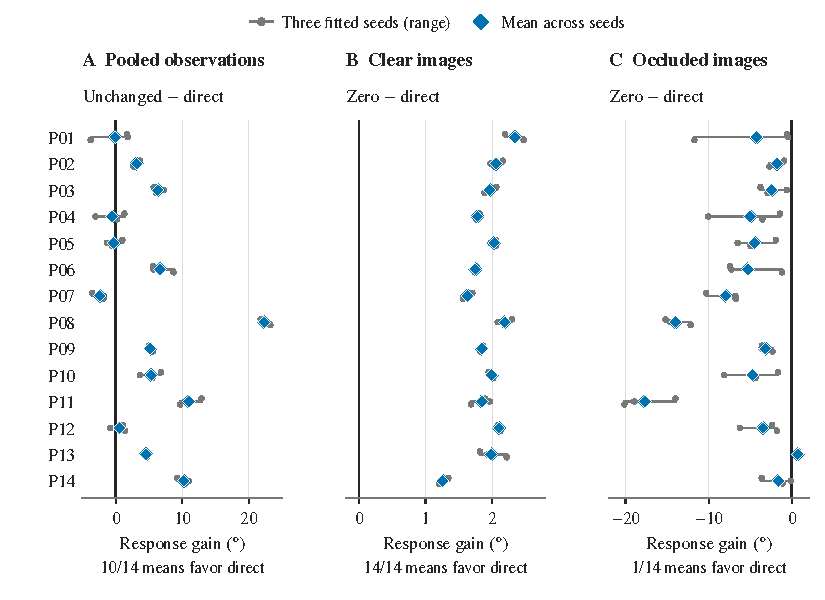
\includegraphics[width=\linewidth]{figures/cases.pdf}
\caption{Participant response profiles, with all 14 development people shown without selection. A: unchanged-minus-direct error, pooled over observations. B--C: zero-minus-direct error for clear and occluded images. Positive values favor jointly fitted direct coordinate restoration. Diamonds average seeds 17, 29, and 43; gray points and horizontal ranges show those fitted values, not confidence intervals. The original 720$\dg$ failure cost and hierarchical aggregation are retained; nonheld/held response strata have 2:1 weighting. Estimators, cameras, naming conditions and physical orientations are pooled. P01--P14 refer to the same people in every panel. Axis ranges differ. These exploratory summaries are not reconstructed poses or clinical examples.}
\label{fig:cases}
\end{figure}
